При исследовании стационарных процессов различной физической природы (колебания, теплопроводность, диффузия, и др.) обычно приходят к уравнениям эллиптического типа. Наиболее распространённым уравнением этого типа является \textit{уравнение Лапласа}
\[
	\Delta u = 0
\]

Функция $u$ называется \textit{гармонической } в области $\Omega$, если она непрерывна в этой области вместе со своими производными до 2-го порядка и удовлетворяет уравнению Лапласа.\\ 


Предcтавления в различных системах координат
\begin{flalign*}
\begin{tabular}{l l}
	\textbf{В декартовой} &$\displaystyle\Delta u = \derp{u}{x}{2} + \derp{u}{y}{2} + \derp{u}{z}{2}$\\[10pt]
	\textbf{В цилиндрической} &$\displaystyle\Delta u = \derp{u}{r}{2} + \frac{1}{r} \derp{u}{r}{} \frac{1}{r} \derp{u}{\theta}{2} + \derp{u}{z}{2}$ \\[10pt]
	\textbf{В сферической} &$\displaystyle\Delta u = \derp{u}{r}{2} + \frac{2}{r} \derp{u}{r}{} + \frac{1}{r^2 \sin \theta} \derp{}{\theta}{} \left(\sin \theta \derp{u}{\theta}{} \right) + \frac{1}{r^2 \sin^2 \theta} \derp{u}{\varphi}{2}$\\
\end{tabular}
\end{flalign*}
Рассмотрим некоторый объём $\Omega$, ограниченный поверхностью $S$. 
\begin{figure}[h!]
	\centering
	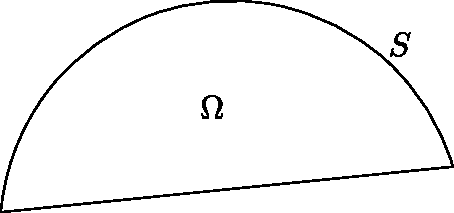
\includegraphics{figElliptic1.pdf}
	\label{fig:elliptic1}
\end{figure}\\
Задача о стационарном распределении температуры $u(x, y, z)$ внутри тела $\Omega$ формулируется следующим образом:\\

\textit{Найти функцию $u(x, y, z)$, удовлетворяющую внутри $\Omega$ уравнению}
\[
	\Delta u = - f(x, y, z)
\]
\textit{и граничному условию, которое может быть взято в одном из следующих видов:}
\begin{flalign*}
	\text{\Rmnum{1}. }&\quad u_g = f(x, y, z) &\mbox{первая краевая задача}\\
	\text{\Rmnum{2}. }&\quad \derp{u}{n}{}  = g (x, y, z)&\mbox{вторая краевая задача}\\
	\text{\Rmnum{3}. }&\quad  \derp{u}{n}{} + \alpha u = h(x, y, z ) &\mbox{третья краевая задача}
\end{flalign*}
\textit{где $f, g,  h$ -- заданные функции, $\derp{u}{n}{}$ --  производная по внешней нормали к поверхности $S$.}\\

Первую краевую задачу называют \textit{задачей Дирихле}, вторую \textit{задачей Неймана}. Третья задача  -- задача \textit{смешанная}. 


%\[
%	\iint\limits_S A_n dS \iiint\limits_{\omega} du A d \omega
%\]
%
%
%\[
%	\bar A = u grad v - v grad u
%\]
%\[
%	A_n =\bar A \cdot \bar n
%\]
%\[
%	A_n = u \bar grad v \bar n - v \bar grad u \cdot \bar n = u \der{v}{n}{} - v \der{u}{n}{}
%\]
